


In my \url{http://procomun.wordpress.com/2012/02/18/maps_with_r_1/} I described how to produce a multivariate
choropleth map with R.  Now I will show how to create a map from
raster files. One of them is a factor which will group the values of
the other one. Thus, once again, I will superpose several groups in
the same map.

First let's load the packages.


\lstset{language=R}
\begin{lstlisting}
library(raster)
library(rasterVis)
library(colorspace)
\end{lstlisting}

Now, I define the geographical extent to be analyzed (approximately India and China).

\lstset{language=R}
\begin{lstlisting}
ext <- extent(65, 135, 5, 55)
\end{lstlisting}

The first raster file is the population density in our planet,
available at this \url{http://neo.sci.gsfc.nasa.gov/Search.html?group%3D64} (choose the Geo-TIFF floating
option, \~{}25Mb).  After reading the data with \texttt{raster} I subset the
geographical extent and replace the 99999 with \texttt{NA}.



\lstset{language=R}
\begin{lstlisting}
pop <- raster('875430rgb-167772161.0.FLOAT.TIFF')
pop <- crop(pop, ext)
pop[pop==99999] <- NA
\end{lstlisting}


\lstset{language=R}
\begin{lstlisting}
pTotal <- levelplot(pop, zscaleLog=10, par.settings=BTCTheme)
pTotal
\end{lstlisting}

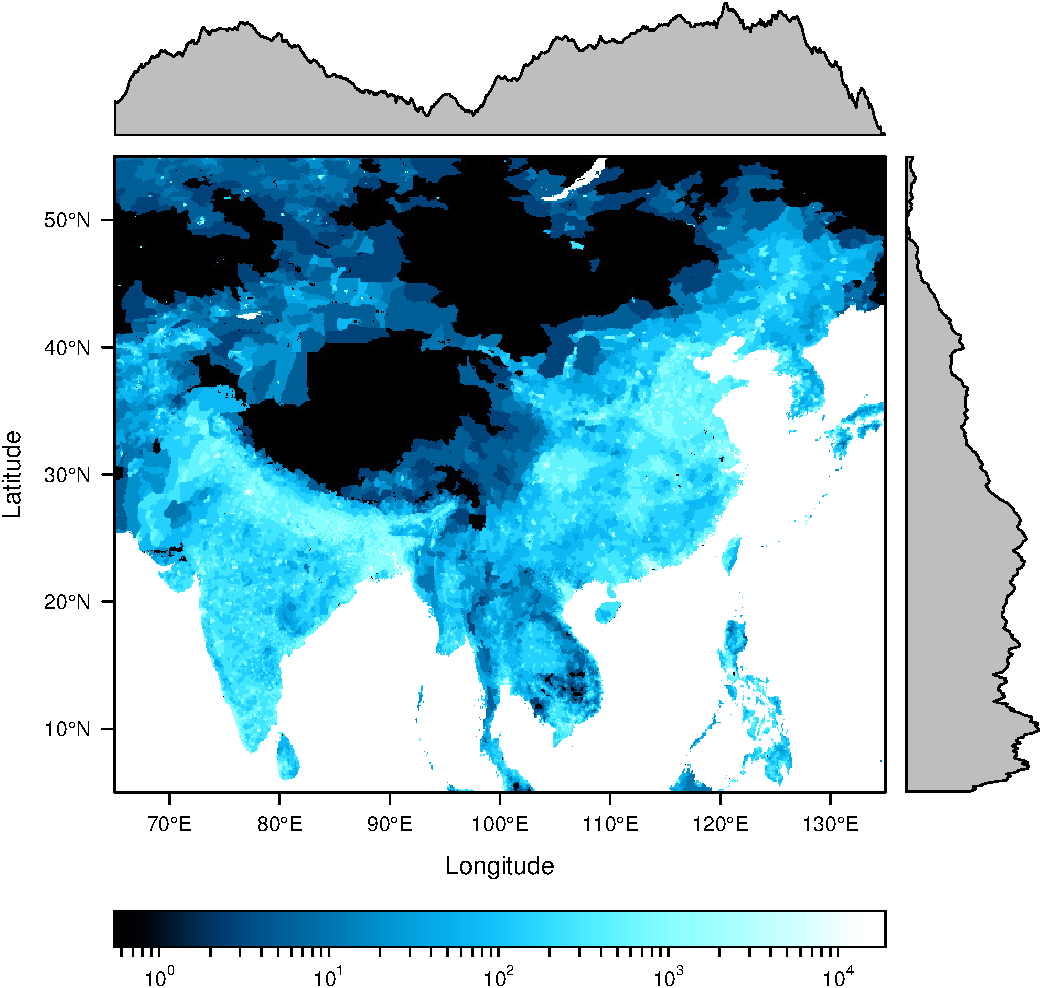
\includegraphics[width=.9\linewidth]{figs/populationNASA.pdf}


The second raster file is the land cover classification (available at this \url{http://neo.sci.gsfc.nasa.gov/Search.html?group%3D20%20})




\lstset{language=R}
\begin{lstlisting}
landClass <- raster('241243rgb-167772161.0.TIFF')
landClass <- crop(landClass, ext)
\end{lstlisting}

The codes of the classification are described \url{http://eoimages.gsfc.nasa.gov/images/news/NasaNews/ReleaseImages/LCC/Images/lcc_key.jpg}. In summary, the
sea is labeled with 0, forests with 1 to 5, shrublands, grasslands and
wetlands with 6 to 11, agriculture and urban lands with 12 to 14, and
snow and barren with 15 and 16.  This four groups (sea is replaced
\texttt{NA}) will be the levels of the factor.


\lstset{language=R}
\begin{lstlisting}
landClass[landClass %in% c(0, 254)] <- NA
landClass <- cut(landClass, c(0, 5, 11, 14, 16))
landClass <- ratify(landClass)
rat <- levels(landClass)[[1]]
rat$classes <- c('Forest', 'Land', 'Urban', 'Snow')
levels(landClass) <- rat
\end{lstlisting}


\lstset{language=R}
\begin{lstlisting}
myTheme <- modifyList(rasterTheme(),# Blue background
                      list(panel.background = list(col='lightskyblue1')))

pal <- c('palegreen4', # Forest
         'lightgoldenrod',              # Land
         'indianred4',                  # Urban
         'snow3')                       # Snow

## pals <- cbind(brewer.pal(n=9, 'Greens'),
##               brewer.pal(n=9, 'Oranges'),
##               brewer.pal(n=9, 'Greys'),
##               brewer.pal(n=9, 'Purples'))
\end{lstlisting}


\lstset{language=R}
\begin{lstlisting}
levelplot(landClass, maxpixels=3.5e5,
          par.settings=myTheme,
          col.regions=pal)
\end{lstlisting}

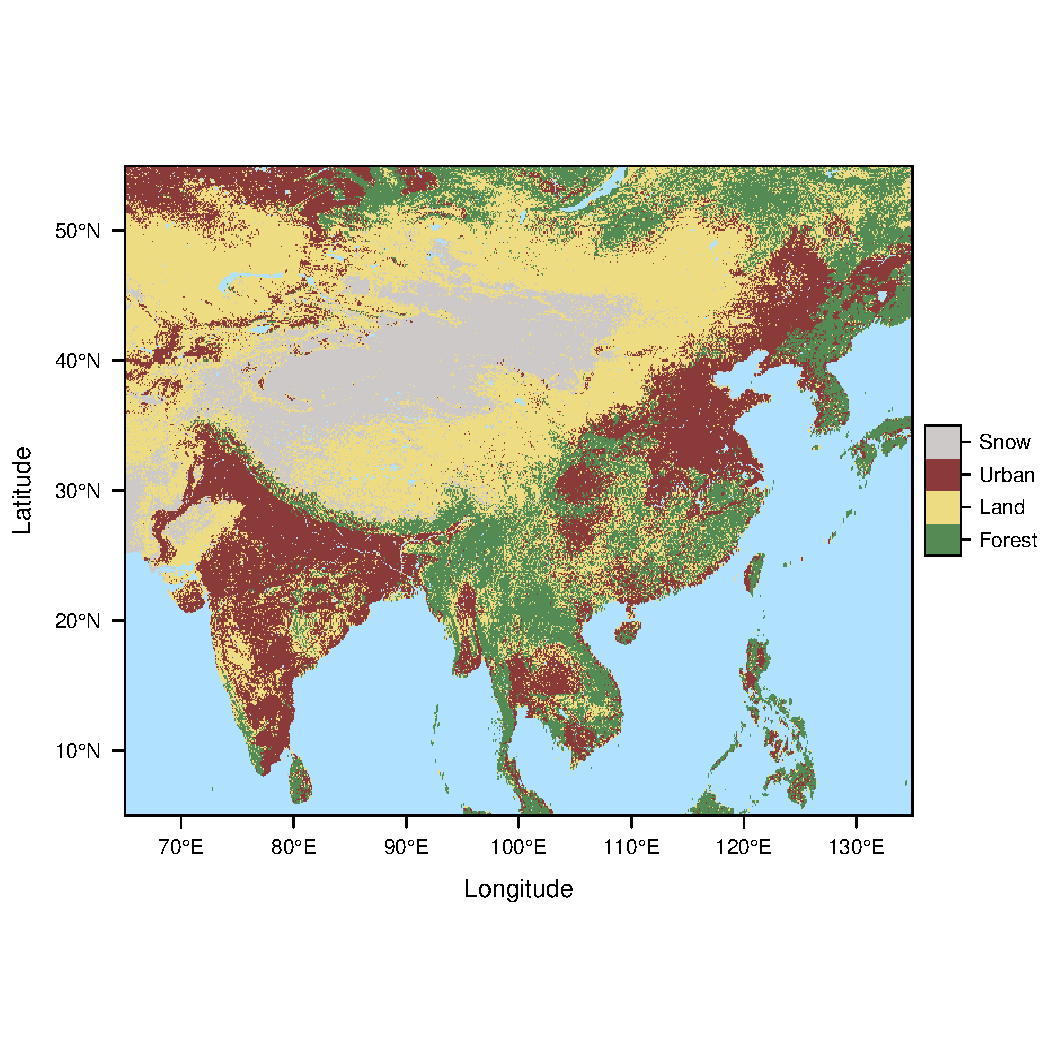
\includegraphics[width=.9\linewidth]{figs/landClass.pdf}

This histogram shows the distribution of the population density in each land class.


\lstset{language=R}
\begin{lstlisting}
s <- stack(pop, landClass)
layerNames(s) <- c('pop', 'landClass')
histogram(~log10(pop)|landClass, data=s,
            scales=list(relation='free'))
\end{lstlisting}

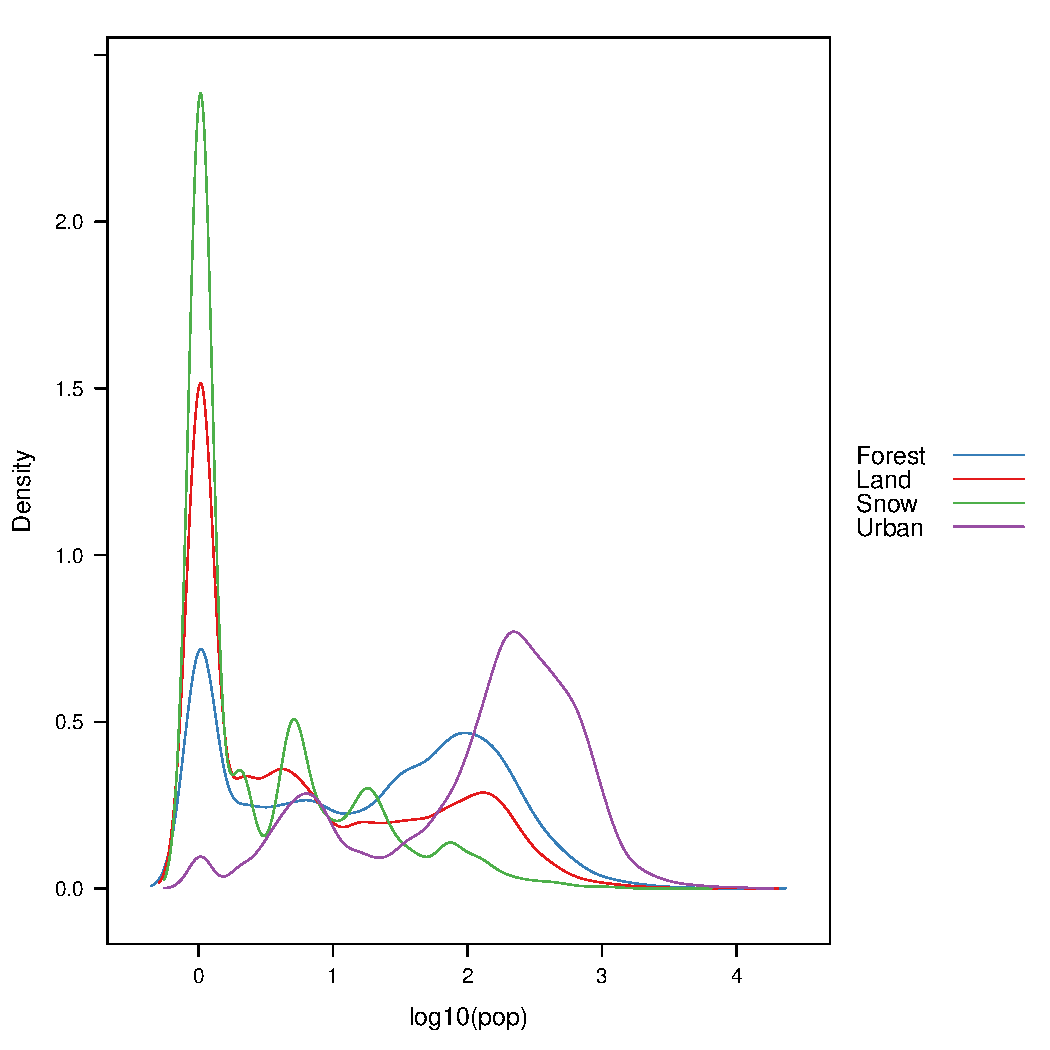
\includegraphics[width=.9\linewidth]{figs/histogramLandClass.pdf}

Everything is ready for the map. I will create a list of \texttt{trellis}
objects with four elements (one for each level of the factor). Each of
these objects is the representation of the population density in a
particular land class.  I use the same scale for all of them to allow
for comparisons. The \texttt{at} argument of levelplot receives the
correspondent \texttt{at} values from the \emph{global} map.


\lstset{language=R}
\begin{lstlisting}
col2hcl <- function(col){
  rgb <- t(col2rgb(col))/256
  luv <- convertColor(rgb, 'sRGB', 'Luv')
  coords <- as(LUV(luv), 'polarLUV')@coords
  coords
  }
\end{lstlisting}


\lstset{language=R}
\begin{lstlisting}
at <- pTotal$legend$bottom$args$key$at
nClasses <- length(rat$classes)

pList <- lapply(1:nClasses, function(i){
  landSub <- landClass
  landSub[!(landClass==i)] <- NA
  popSub <- mask(pop, landSub)

##  cols <- colorRampPalette(c('white', pal[i]),  space='Lab')(100)
  hclPal <- col2hcl(pal[i])
  cols <- rev(sequential_hcl(100, h=hclPal[1], c=c(hclPal[2], 0), l=c(hclPal[3], 90)))

  pClass <- levelplot(popSub, zscaleLog=10, at=at, maxpixels=3.5e5,
                      col.regions=cols, margin=FALSE)
})
\end{lstlisting}


\lstset{language=R}
\begin{lstlisting}
m <- matrix(1:nClasses, nrow=2)
for (i in 1:nClasses){
    print(update(pList[[i]], main=rat$classes[i]),
          split=c(col(m)[i], row(m)[i], 2, 2),
          more=(i<nClasses))
  }
\end{lstlisting}

\includegraphics[width=.9\linewidth]{figs/pop_landClass_panels.pdf}

And that's all. The rest of the code is exactly the same as in \url{http://procomun.wordpress.com/2012/02/18/maps_with_r_1/}. If you execute it you will get this image (click on it
for higher resolution).





